% begin module cycloid-equations-ex7
\begin{frame}
\begin{example} %[Example 7, p. 660]
Find parametric equations of a cycloid made using a circle with radius $r$ that rolls along the $x$-axis such that $P$ hits the origin.
\begin{columns}[c]
\column{.4\textwidth}

\psset{xunit=1.6cm, yunit=1.6cm}
\begin{pspicture}( -0.6, -0.6)(2.65,2.3)
\psframe*[linecolor=white](-0.6, -0.6)(2.65,2.3)
\tiny%
\psaxes[arrows=<->, ticks=none, labels=none ](0,0)( -0.500000, -0.5)(2.55,2.2)%
\parametricplot[linecolor=\fcColorTangent, plotpoints=1000, algebraic=true]{0}{6.283185307}{cos(t)+1.256637061|sin(t)+1}%
\uncover<2->{%
\psplot[linecolor=green, plotpoints=300]{0.305581} {1.256637061} {1 1 -1.25664 x add 2 exp -1 mul add 0.5 exp -1 mul add }%
}%
%Calculator input: plotCurve{}(- \sin{}t+t, - \cos{}t+1, 0, \pi)
\parametricplot[linecolor=\fcColorGraph, plotpoints=1000] { 0}{2.8}{t t 57.29578 mul sin -1 mul add 1 t 57.29578 mul cos -1 mul add }

\fcFullDot{0.305581}{0.690983}
\rput[r](0.2, 0.69){$P$}
\fcFullDot{1.256637061}{1}
\rput[bl](1.286637061,1.05){\uncover<5->{\alertNoH{5}{$ C=(r\theta,r)$}}}

\uncover<6->{\psline[linestyle=dashed](0.305581,0)(0.305581,0.690983)
\rput[b](0.15, 0.05){\alertNoH{6}{$x$}}
\rput[l](0.32, 0.35){\alertNoH{6}{$y$}}
}

\psline(0.305581,0.690983)(1.256637061,1)
\rput[b](0.75, 0.85){$r$}

\uncover<7->{
\psline[linestyle=dashed](0.305581,0.690983)(1.256637061,0.690983)
\psline(1.156637061,0.690983)(1.156637061,0.590983)(1.256637061,0.590983)
\rput[l](1.306637061,0.690983){$Q$}
}

\psline(1.256637061,0.1)(1.356637061,0.1)(1.356637061,0)
\rput[lt](1.256637061,-0.1){$T$}
\psline(1.256637061,1)(1.256637061,0)

\uncover<3->{\psline[linecolor=green](0,0)(1.256637061, 0)}

\uncover<4->{
\psline{<-}(0,-0.2)(0.5, -0.2)
\psline{->}(0.72,-0.2)(1.256637061, -0.2)
\rput(0.62, -0.2){\alertNoH{4}{$r\theta$}}
}
\rput(1.2, 0.9){\uncover<2->{\alertNoH{2}{$\theta$}}}
\rput (-0.2, -0.2){$O$}
\end{pspicture}

%\ \only<handout:0| -2>{%
%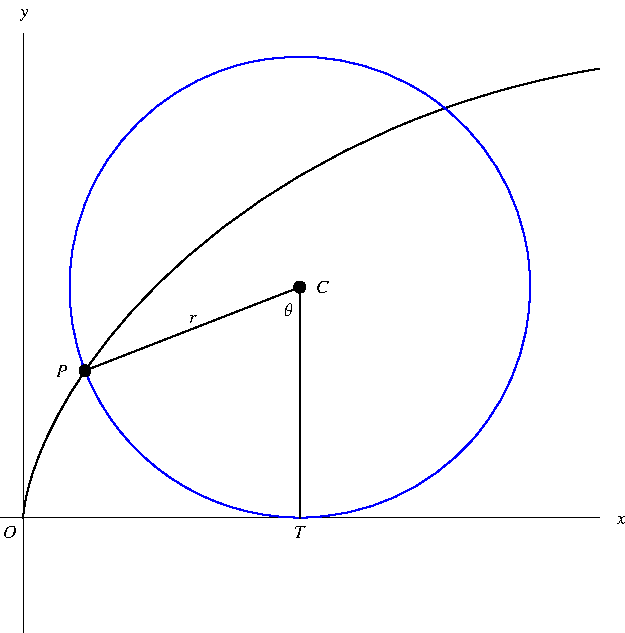
\includegraphics[width=5cm]{parametric-curves/pictures/11-01-cycloideqa.pdf}%
%}%
%\only<handout:0| 3>{%
%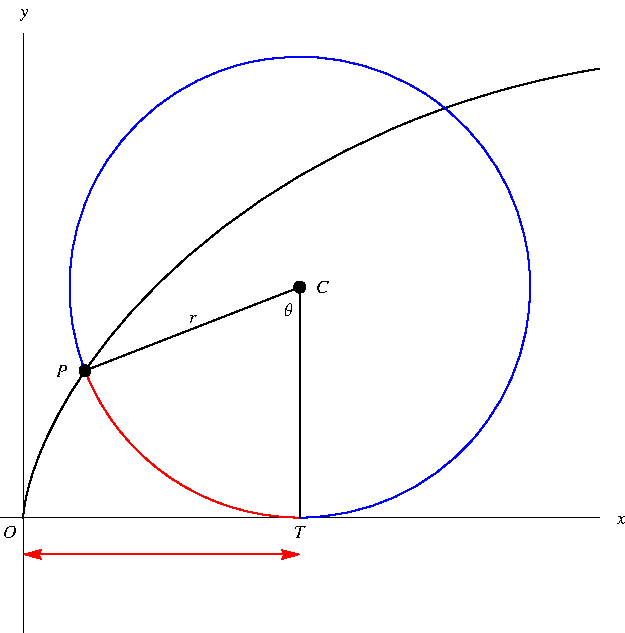
\includegraphics[width=5cm]{parametric-curves/pictures/11-01-cycloideqb.pdf}%
%}%
%\only<handout:0| 4>{%
%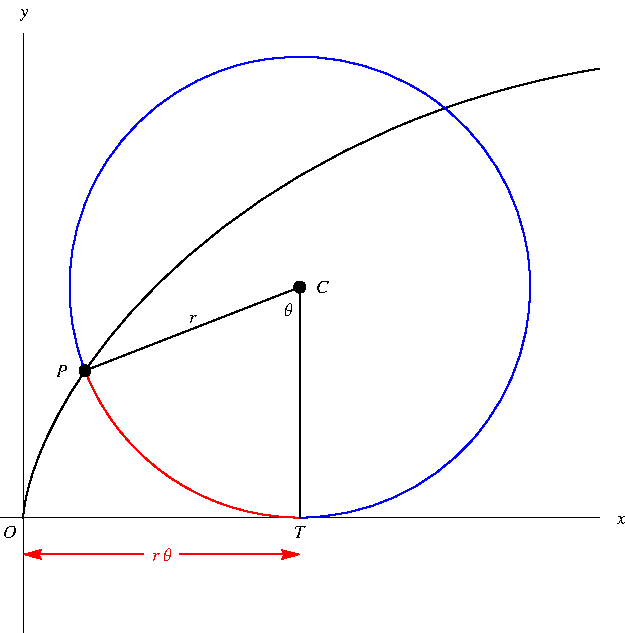
\includegraphics[width=5cm]{parametric-curves/pictures/11-01-cycloideqc.pdf}%
%}%
%\only<handout:0| 5>{%
%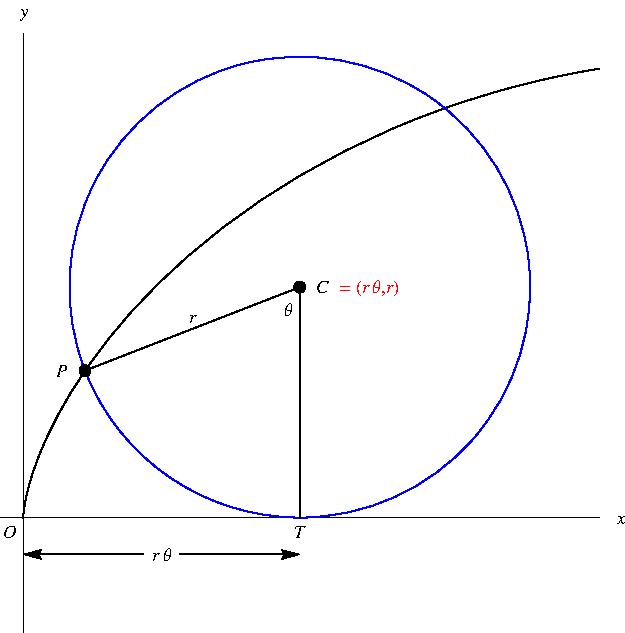
\includegraphics[width=5cm]{parametric-curves/pictures/11-01-cycloideqd.pdf}%
%}%
%\only<handout:0| 6>{%
%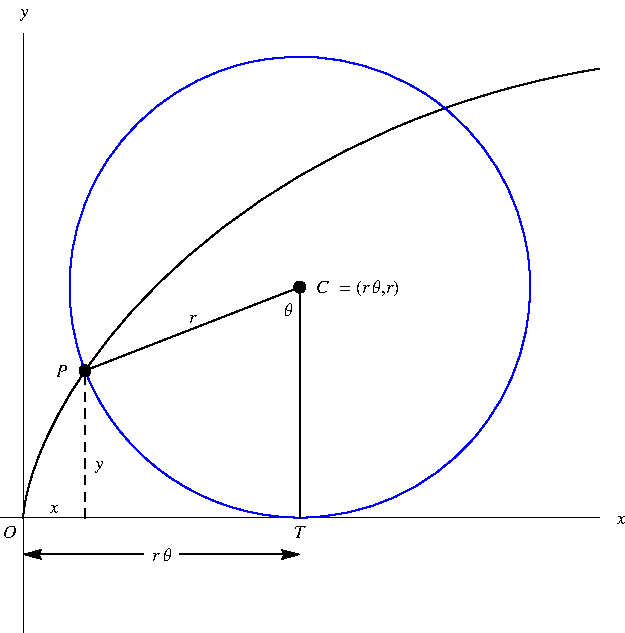
\includegraphics[width=5cm]{parametric-curves/pictures/11-01-cycloideqe.pdf}%
%}%
%\only<7->{%
%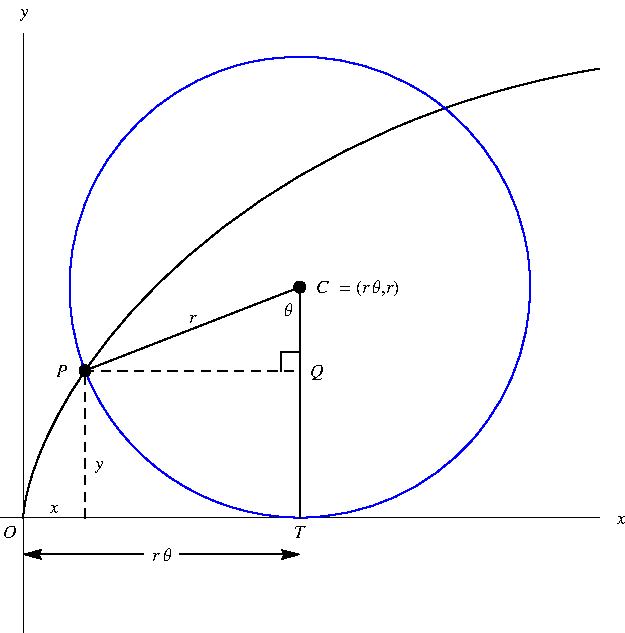
\includegraphics[width=5cm]{parametric-curves/pictures/11-01-cycloideqf.pdf}%
%}%
\column{.6\textwidth}
\begin{itemize}
\item<2->  We choose our parameter to be \alertNoH{2}{$\theta$}, the angle of rotation of the circle.
\item<3->  How far has the circle moved if it has rolled through $\theta$ radians?
\abovedisplayskip=0pt
\belowdisplayskip=0pt
\[
\uncover<3->{%
{|OT|} = \alertNoH{ 4}{{ \textrm{arc} PT} }%
}%
\uncover<4->{%
\alertNoH{ 4}{ = r\theta}%
}%
\]
\item<5->  Then the center is $\alertNoH{5}{C = (r\theta , r)}$.
\item<6->  Let the coordinates of $P$ be $(x,y)$.
\end{itemize}
\[
\begin{array}{cccccc}
\uncover<6->{%
\alertNoH{ 8}{x}%
}&%
\uncover<6->{%
\alertNoH{ 8}{=}%
}&%
\uncover<8->{%
\alertNoH{ 8}{\alertNoH{ 9-10}{|OT|} - \alertNoH{ 11-12}{|PQ|}}%
}&%
\uncover<9->{%
=%
}&%
\uncover<10->{%
\alertNoH{ 10}{r\theta}%
}%
\uncover<9->{-}%
\uncover<12->{%
\alertNoH{ 12}{r\sin \theta}%
}\\%

\uncover<6->{%
\alertNoH{ 13}{y}%
}&%
\uncover<6->{%
\alertNoH{ 13}{=}%
}&%
\uncover<13->{%
\alertNoH{ 13}{\alertNoH{ 14-15}{|CT|} - \alertNoH{ 16-17}{|CQ|}}%
}&%
\uncover<14->{%
=%
}&%
\uncover<15->{%
\alertNoH{ 15}{r}%
}%
\uncover<14->{-}%
\uncover<17->{%
\alertNoH{ 17}{r\cos \theta}%
}\\%
\end{array}
\]
\end{columns}
\uncover<18->{%
Therefore the equations are
\abovedisplayskip=0pt
\belowdisplayskip=0pt
\[
x = r(\theta - \sin \theta ),\qquad y = r(1-\cos \theta ),\qquad \theta \in \mathbb{R}
\]
}%
\end{example}
\end{frame}
% end module cycloid-equations-ex7
